% !TeX root = ../../main.tex
\subsection{Data Storage \& Management}\label{sec:storage}
\begingroup
% Đánh số bảng/hình theo mục (2.x.y), giống Transaction.
\setcounter{table}{0}\setcounter{figure}{0}
\renewcommand{\thetable}{\thesubsection.\arabic{table}}
\renewcommand{\thefigure}{\thesubsection.\arabic{figure}}
\renewcommand{\theHtable}{\thesubsection.\arabic{table}}
\renewcommand{\theHfigure}{\thesubsection.\arabic{figure}}
\subsubsection{Mục tiêu và phạm vi so sánh}

Trong các hệ thống thương mại điện tử hiện đại, việc lựa chọn và kết hợp các hệ quản trị cơ sở dữ liệu đóng vai trò then chốt nhằm cân bằng giữa tính toàn vẹn dữ liệu nghiệp vụ và hiệu năng truy vấn ứng dụng. Trong kiến trúc của hệ thống ShopFlash, phân hệ lưu trữ dữ liệu danh mục được thiết kế theo mô hình kết hợp giữa Oracle Database và Redis. Trong đó, Oracle đóng vai trò là cơ sở dữ liệu nghiệp vụ gốc, chịu trách nhiệm lưu trữ bền vững các thực thể \texttt{CATEGORIES}, \texttt{PRODUCTS} và \texttt{PRODUCT\_INVENTORY}. Ngược lại, Redis được khai thác như một lớp bộ nhớ đệm đóng vai trò lưu trữ bản chiếu sản phẩm nhằm tối ưu hóa tốc độ đọc và hỗ trợ truy vấn nhanh.

Mục tiêu so sánh ở phần này không nhằm tìm ra một hệ quản trị cơ sở dữ liệu vượt trội hoàn toàn về mọi mặt, mà tập trung xác định rõ sự phân công trách nhiệm phù hợp giữa một cơ sở dữ liệu quan hệ truyền thống và một cơ sở dữ liệu lưu trữ trên bộ nhớ trong đối với một ứng dụng có quan hệ dữ liệu phức tạp. Cần lưu ý rằng, hệ thống ShopFlash thực tế còn chứa nhiều bảng nghiệp vụ khác (như người dùng, đơn hàng, thanh toán); tuy nhiên, các thử nghiệm dưới đây chỉ tập trung phạm vi đo lường trên phân hệ danh mục sản phẩm. Các số liệu thực nghiệm được thu thập từ một ảnh chụp dữ liệu thực tế sau khi dựng lại danh mục ShopFlash với 100 \texttt{Category}, 1\,000 \texttt{Product} và 1\,000 bản ghi \texttt{ProductInventory}.

\subsubsection{Kiến trúc lưu trữ của Oracle và Redis}

Để có cơ sở đánh giá thực nghiệm mô hình lưu trữ, cần xem xét bản chất kiến trúc và cơ chế tổ chức dữ liệu nền tảng của hai hệ quản trị cơ sở dữ liệu.

\paragraph{Oracle Database}

Oracle áp dụng mô hình dữ liệu quan hệ với cơ chế lưu trữ bền vững trên đĩa cứng \cite{oracleLogicalStorage}. Về mặt lưu trữ logic, dữ liệu bảng và chỉ mục được tổ chức theo cấu trúc phân cấp từ trên xuống dưới:

\begin{itemize}[label=--]
    \item \textbf{Data Block:} Đơn vị I/O nhỏ nhất của Oracle (thường là 8 KB), chứa các dòng dữ liệu thực tế cùng thông tin quản lý header và không gian trống dành cho việc cập nhật dòng \cite{oracleLogicalStorage}.
    
    \item \textbf{Extent:} Tập hợp các data block liên tục được cấp phát trong một lần mở rộng không gian lưu trữ, giúp giảm chi phí cấp phát đĩa cứng khi dữ liệu phát triển \cite{oracleLogicalStorage}.
    
    \item \textbf{Segment:} Tập hợp các extent dành riêng cho một đối tượng cơ sở dữ liệu cụ thể như \texttt{TABLE segment}, \texttt{INDEX segment} hoặc \texttt{LOB segment}. Dữ liệu của một segment có thể trải dài trên nhiều datafile khác nhau \cite{oracleLogicalStorage}.
\end{itemize}

\begin{figure}[htbp]
    \centering
    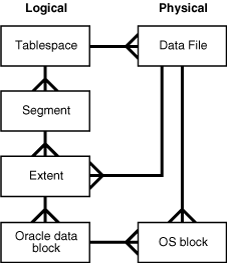
\includegraphics[width=0.4\textwidth]{Pictures/Task_1/oracle-logical-storage.png}
    \caption{Cấu trúc lưu trữ logic và vật lý (Nguồn: Oracle Database Concepts \cite{oracleLogicalStorage}).}
    \label{fig:st-oracle-logical-physical-storage}
\end{figure}

Mô hình lưu trữ đĩa cứng kết hợp với Redo Log, Database Buffer Cache và cơ chế kiểm soát giao dịch ACID giúp Oracle duy trì tính toàn vẹn dữ liệu nghiêm ngặt, hỗ trợ khôi phục sau sự cố và đảm bảo khả năng mở rộng cho hệ thống \cite{oracleLogicalStorage}.

\paragraph{Redis}

Khác với Oracle, Redis là một cơ sở dữ liệu NoSQL dạng key-value hoạt động hoàn toàn trên bộ nhớ trong \cite{redisDataTypes}.
\begin{itemize}[label=--]
    \item \textbf{In-memory Keyspace và bộ cấp phát bộ nhớ:} Toàn bộ dữ liệu được tổ chức dưới dạng keyspace và duy trì trực tiếp trong RAM. Redis sử dụng bộ cấp phát \texttt{jemalloc} để quản lý các khối RAM và tối ưu hóa memory overhead. Để bảo vệ bộ nhớ, hệ thống hỗ trợ các eviction policy như \texttt{allkeys-lru} khi vượt quá ngưỡng \texttt{maxmemory}.
    
    \item \textbf{Cấu trúc RedisJSON:} Phân hệ mở rộng RedisJSON nâng cấp Redis thành một document store. Dữ liệu JSON được phân tích cú pháp và lưu trữ dưới dạng cấu trúc cây binary trong RAM, cho phép truy xuất và sửa đổi các nested field với độ phức tạp $O(1)$ hoặc $O(N)$ mà không cần encode hoặc decode lại toàn bộ chuỗi văn bản \cite{redisJson}.
    
    \item \textbf{Cơ chế Persistence:} Mặc dù hoạt động trên RAM, Redis hỗ trợ hai cơ chế ghi đĩa bền vững bao gồm tạo snapshot RDB (Redis Database Backup) và ghi nhật ký AOF (Append-Only File) \cite{redisPersistence}.
\end{itemize}

Tuy nhiên, cấu trúc lưu trữ của Redis không tự động quản lý các mối quan hệ liên kết như foreign key giữa các document, cũng như không tự động áp dụng các ràng buộc schema ở cấp độ cơ sở dữ liệu.

\paragraph{So sánh tổng quan kiến trúc}

Sự khác biệt về kiến trúc lưu trữ tạo ra tính chất kỹ thuật đối lập giữa hai hệ thống: Oracle tập trung vào tính toàn vẹn, tính bền vững và đóng vai trò là source of truth nghiêm ngặt; trong khi Redis tối ưu triệt để cho hiệu năng đọc ghi tốc độ cao với độ trễ sub-millisecond. Sự kết hợp cả hai hệ thống trong ShopFlash chính là bài toán khai thác ưu điểm kiến trúc của từng phía.

\subsubsection{Thiết kế lưu trữ trong kiến trúc ShopFlash}

Oracle đóng vai trò là source of truth. Ba bảng \texttt{CATEGORIES}, \texttt{PRODUCTS} và \texttt{PRODUCT\_INVENTORY} chứa dữ liệu catalog, quan hệ Category--Product và tồn kho. Product có foreign key tới Category; SKU và slug có unique constraint; giá và số lượng tồn kho được bảo vệ thêm bằng check constraint \cite{oracleConstraints}. Bảng ProductInventory tách khỏi Product để luồng Storage chỉ cập nhật \texttt{on\_hand\_quantity}, còn số lượng đã giữ cho Flash Sale thuộc module concurrency.

Redis không lưu một bản sao đầy đủ của mô hình quan hệ. Với mỗi Product, backend tạo một RedisJSON document có key \texttt{product:\{id\}} gồm các trường \texttt{id}, \texttt{sku}, \texttt{name}, \texttt{categoryId}, \texttt{categoryName}, \texttt{price}, \texttt{status}, \texttt{inStock} và \texttt{thumbnailUrl}. Category, Inventory, foreign key và unique SKU không được Redis sở hữu. Mọi thao tác CRUD đi qua Oracle bằng JDBC; chỉ sau khi transaction Oracle commit thành công, backend mới cập nhật product projection Redis. Khi Redis lỗi, Oracle không rollback; projection có thể được dựng lại từ Oracle.

\begin{table}[H]
    \centering
    \caption{Trách nhiệm dữ liệu của Oracle và Redis trong ShopFlash}
    \label{tab:st-storage-model-mapping}
    \begin{tabularx}{\textwidth}{@{}p{0.24\textwidth}XX@{}}
        \toprule
        Thành phần & Oracle & Redis \\
        \midrule
        Category & Dòng trong \texttt{CATEGORIES}; là dữ liệu gốc. & Không có Category document độc lập. \\
        Product & Dòng trong \texttt{PRODUCTS}; là dữ liệu gốc. & Document phái sinh \texttt{product:\{id\}}. \\
        Inventory & \texttt{PRODUCT\_INVENTORY}, có version để optimistic locking. & Chỉ suy ra \texttt{inStock} trong product projection. \\
        Quan hệ và ràng buộc & Foreign key Product--Category, unique SKU/slug, check constraint giá và tồn kho. & Không có foreign key, unique hay check constraint khai báo. \\
        Đồng bộ & Commit transaction trước. & Cập nhật sau commit; có API rebuild khi projection stale. \\
        \bottomrule
    \end{tabularx}
\end{table}

\subsubsection{Đánh giá thực nghiệm}

\paragraph{Toàn vẹn dữ liệu (E1)}

\noindent\textbf{Phương pháp}\par

Màn hình so sánh Oracle–Redis liệt kê các ràng buộc được bảo vệ ở form API và Oracle. Để chứng minh RedisJSON không có constraint khai báo tương đương, backend tạo một document kiểm thử có \texttt{categoryId = 999999999} (không tham chiếu Category Oracle nào) và \texttt{price = -1} (vi phạm điều kiện \texttt{base\_price >= 0} của Oracle). Document này được ghi trực tiếp vào key ngẫu nhiên \texttt{storage-lab:constraint-demo:\{uuid\}}, đọc lại bằng \texttt{JSON.GET}, rồi xóa bằng \texttt{UNLINK} ngay trong cùng request. Key kiểm thử không có prefix \texttt{product:}, nên không đi vào product projection hoặc Redis search index. Thử nghiệm không ghi Oracle và không làm thay đổi dữ liệu Category hoặc Product thật.

\noindent\textbf{Kết quả và phân tích}\par
Hình~\ref{fig:st-storage-lab-integrity} cho thấy RedisJSON nhận document không hợp lệ. Đây không phải lỗi của Redis; RedisJSON là document store linh hoạt và không tự kiểm tra foreign key hay check condition của schema Oracle. Trong kiến trúc ShopFlash, client không được ghi trực tiếp vào Redis: request hợp lệ phải qua API, Oracle là lớp thực thi ràng buộc cuối cùng, còn Redis chỉ nhận projection đã được backend tạo.

\begin{figure}[H]
    \centering
    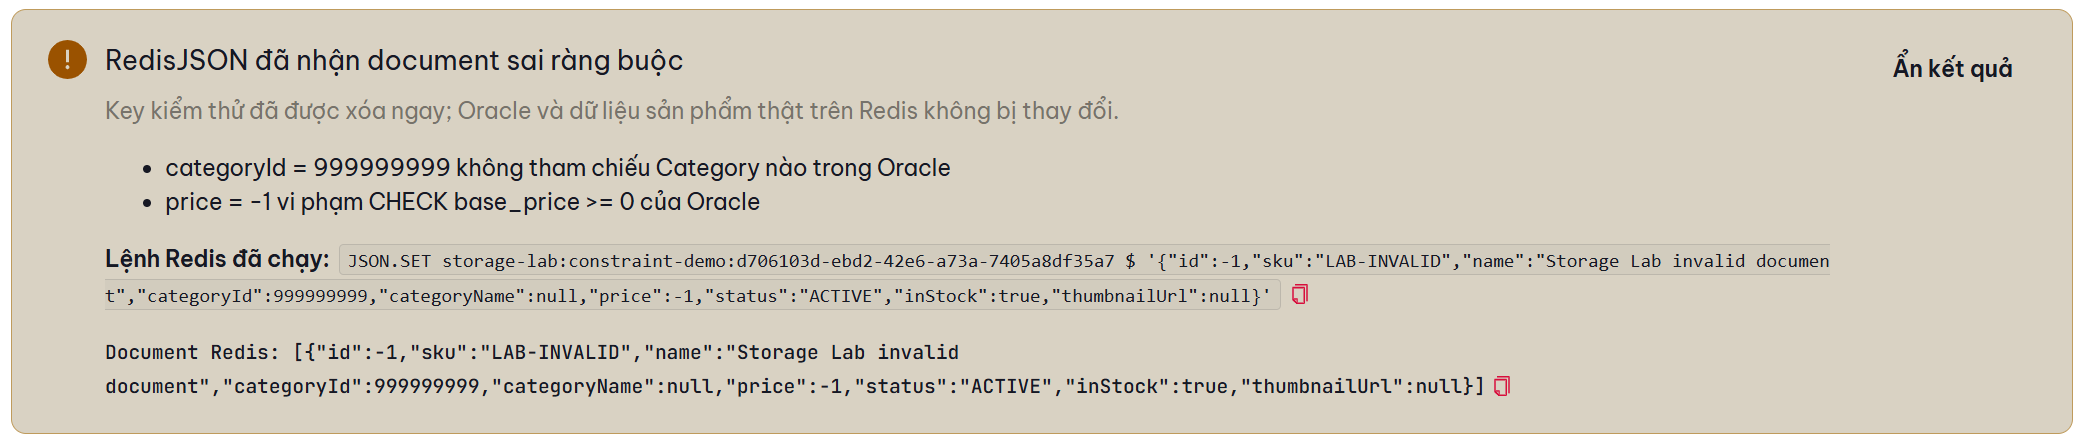
\includegraphics[width=0.8\textwidth]{Pictures/Task_1/storage-lab-constraint-demo.png}
    \caption{E1: RedisJSON nhận document có Category không tồn tại và giá âm; key kiểm thử được dọn ngay sau khi đọc.}
    \label{fig:st-storage-lab-integrity}
\end{figure}

\begin{table}[H]
    \centering
    \caption{Kết luận E1 trong kiến trúc ShopFlash}
    \label{tab:st-integrity-results}
    \begin{tabularx}{\textwidth}{@{}p{0.3\textwidth}XX@{}}
        \toprule
        Quy tắc & Oracle (source of truth) & Redis projection \\
        \midrule
        Category phải tồn tại & Foreign key \texttt{PRODUCTS.category\_id} chặn dữ liệu mồ côi. & Document ghi trực tiếp vẫn có thể chứa \texttt{categoryId} không tồn tại. \\
        SKU không trùng & Unique constraint và kiểm tra của API. & Không dùng làm nơi kiểm tra unique SKU. \\
        Giá không âm & \texttt{CHECK (base\_price >= 0)} và validation API. & Document ghi trực tiếp vẫn có thể chứa \texttt{price = -1}. \\
        Tồn kho không thấp hơn phần đã giữ & Check constraint trên ProductInventory, API kiểm tra và optimistic locking. & Chỉ nhận trường \texttt{inStock} đã suy ra; không quản lý số lượng gốc. \\
        \bottomrule
    \end{tabularx}
\end{table}

\paragraph{Dung lượng lưu trữ (Footprint) (E2)}

\noindent\textbf{Phương pháp}\par
Endpoint \texttt{GET /api/admin/catalog/storage-footprint} đọc \texttt{USER\_}\allowbreak\texttt{SEGMENTS} cho ba table segment và các index segment liên quan trực tiếp đến \texttt{CATEGORIES}, \texttt{PRODUCTS}, \texttt{PRODUCT\_INVENTORY}. Các bảng khác trong cơ sở dữ liệu hệ thống ShopFlash không nằm trong phạm vi tính toán của thử nghiệm này. Tổng dung lượng của Oracle vì thế là dung lượng đã cấp phát (allocated bytes) dành riêng cho phân hệ danh mục catalog, không phải số byte dữ liệu thực tế đang sử dụng của toàn bộ cơ sở dữ liệu. Oracle cấp phát không gian theo extent và thường giữ lại dung lượng đã cấp để tái sử dụng sau khi xóa dòng \cite{oracleLogicalStorage}.

Ở phía Redis, endpoint quét đúng các key \texttt{product:*} và cộng kết quả từ lệnh \texttt{MEMORY USAGE} của từng key \cite{redisMemoryUsage}. Lệnh này trả về lượng bộ nhớ tính bằng byte của một key cùng giá trị đi kèm. Số liệu của Redis không bao gồm bộ nhớ nền của Redis server, Docker container hay bộ nhớ của RediSearch index. Vì vậy, thử nghiệm E2 thực chất so sánh footprint vận hành của dữ liệu gốc trên Oracle với product projection trên Redis, không phải so sánh hai mô hình dữ liệu tương đương hoàn toàn.

\noindent\textbf{Kết quả và phân tích}\par
Sau khi gọi rebuild projection, Oracle có 1\,000 Product và Redis có 1\,000 document; trạng thái projection hoàn toàn đồng bộ. Bảng~\ref{tab:st-storage-footprint-results} ghi lại snapshot thu được từ Storage Lab.

\begin{table}[H]
    \centering
    \caption{Snapshot footprint với 100 Category và 1\,000 Product}
    \label{tab:st-storage-footprint-results}
    \begin{tabularx}{\textwidth}{@{}X r r@{}}
        \toprule
        Hệ / Phạm vi đo & \multicolumn{1}{c}{Dung lượng (bytes)} & \multicolumn{1}{c}{Bytes trên một Product/document} \\
        \midrule
        Oracle: 3 table và index catalog đã cấp phát & 1\,245\,184 & 1\,245.18 \\
        Redis: Các RedisJSON key \texttt{product:*} & 575\,000 & 575.00 \\
        \bottomrule
    \end{tabularx}
\end{table}

Chi tiết segment Oracle trong Hình~\ref{fig:st-storage-lab-segments} cho thấy ba table segment chiếm 458\,752 bytes; các index segment (bao gồm cả LOB index của cột mô tả Product) chiếm 786\,432 bytes. Dung lượng allocated của Oracle lớn hơn Redis projection 670\,184 bytes trong snapshot này. Kết quả này phản ánh đúng vai trò khác nhau giữa hai hệ thống: Oracle lưu dữ liệu gốc, thông tin tồn kho cùng nhiều chỉ mục để đảm bảo tính toàn vẹn và hỗ trợ truy vấn; trong khi Redis chỉ lưu trữ document projection để phục vụ đọc nhanh.

\begin{figure}[H]
    \centering
    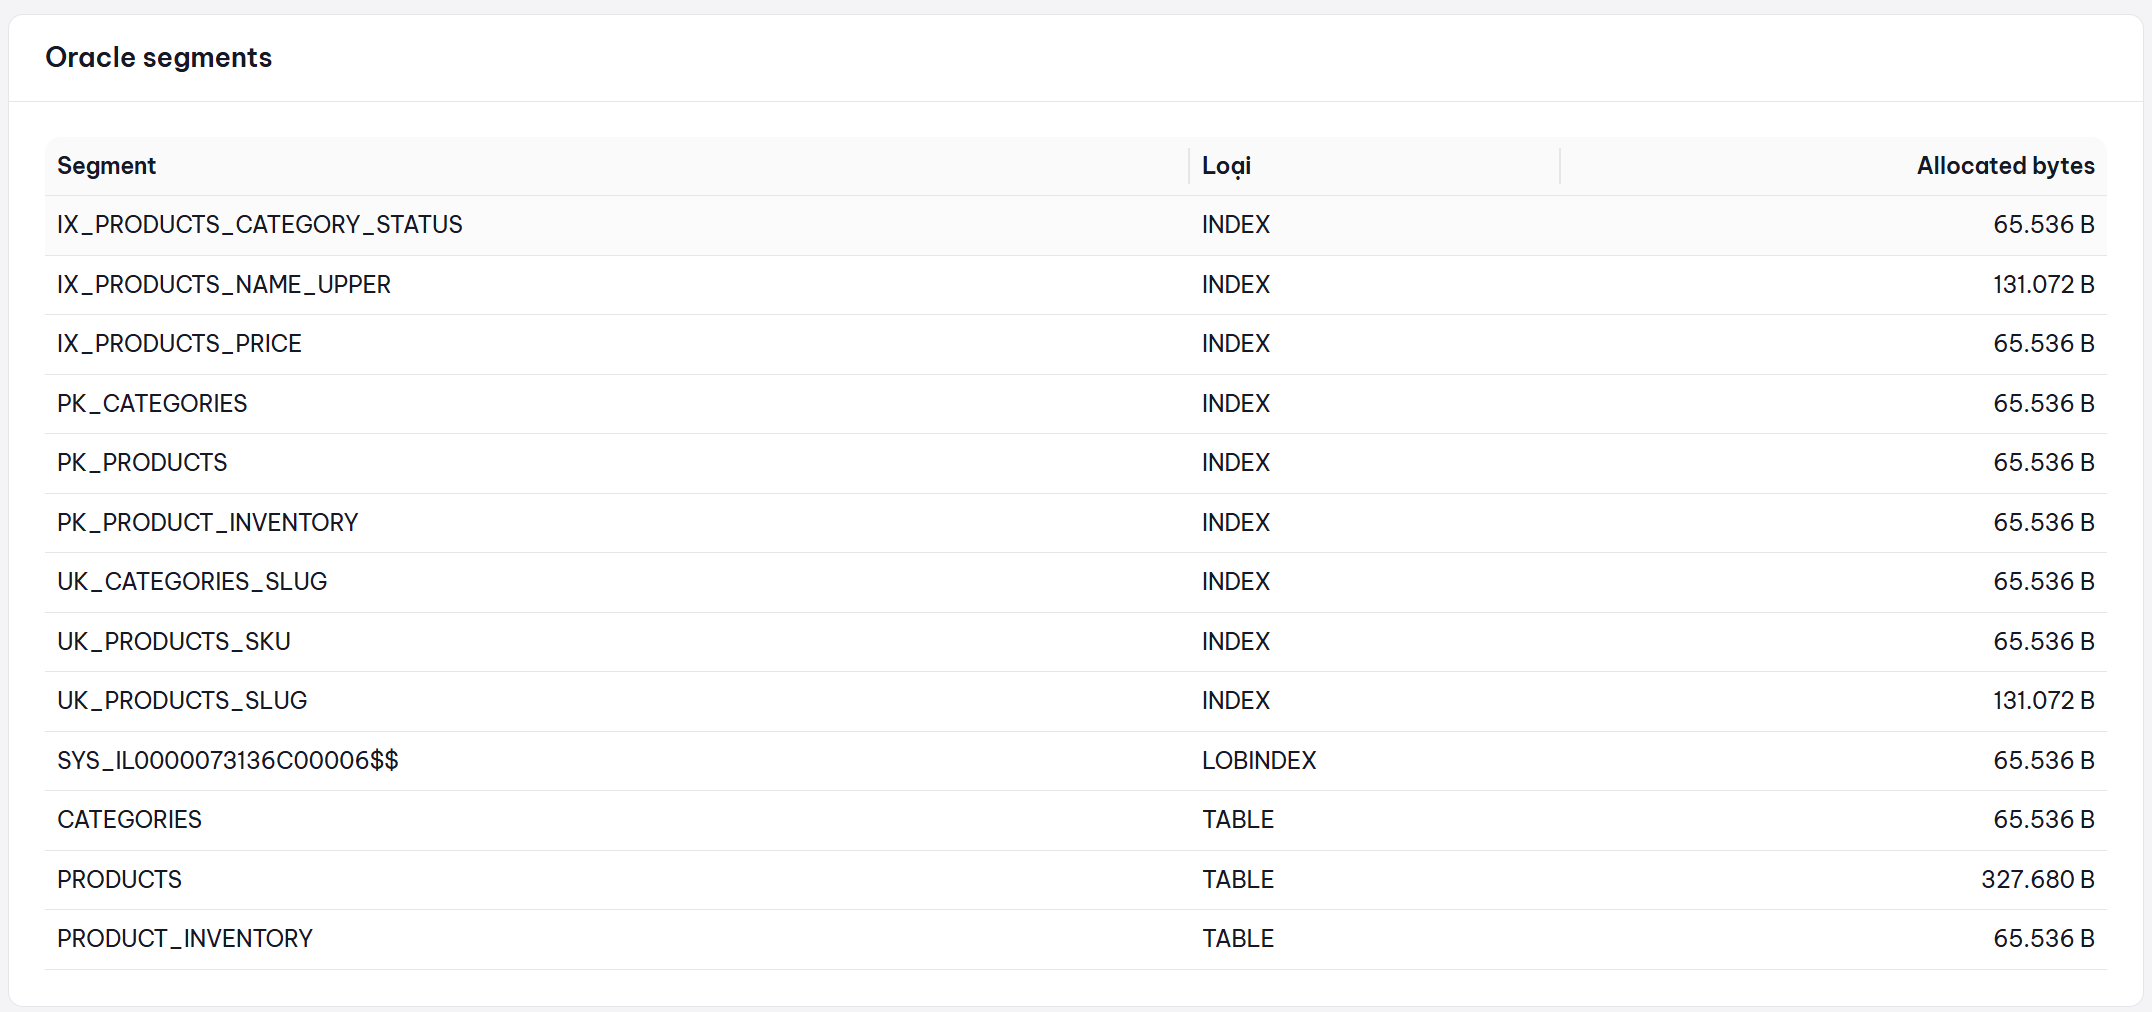
\includegraphics[width=\textwidth]{Pictures/Task_1/storage-lab-segments.png}
    \caption{Các Oracle table và index segment được cộng vào footprint E2.}
    \label{fig:st-storage-lab-segments}
\end{figure}

Số liệu thực nghiệm này không dùng để suy rộng rằng Redis luôn tốn ít dung lượng hơn Oracle trong mọi trường hợp. Kết quả thực tế phụ thuộc vào bản chất dữ liệu, cấu trúc schema, số lượng chỉ mục, cơ chế cấp phát block hoặc extent của Oracle và cách thiết kế cấu trúc JSON trong Redis.

\subsubsection{Đánh giá tổng hợp và định hướng sử dụng DBMS}

Kết quả thực nghiệm E1 và E2 thể hiện rõ sự đánh đổi kỹ thuật giữa hai hệ quản trị cơ sở dữ liệu trong hệ thống ShopFlash:

\begin{itemize}[label=--]
    \item \textbf{Oracle Database} thể hiện ưu thế tuyệt đối ở vai trò source of truth nhờ cơ chế quản lý giao dịch ACID nghiêm ngặt và khả năng cưỡng chế các ràng buộc toàn vẹn ngay tại cấp độ cơ sở dữ liệu. Mặc dù chi phí footprint lưu trữ ban đầu cao hơn do phải duy trì các cấu trúc phân cấp (block, extent, segment) cùng chỉ mục phục vụ ràng buộc, đây là chi phí bắt buộc để bảo vệ tính chính xác của dữ liệu nghiệp vụ gốc.
    \item \textbf{Redis} đạt hiệu quả cao ở luồng đọc nhờ cấu trúc dữ liệu tối ưu trực tiếp trên bộ nhớ trong, giúp giảm footprint trên từng document phái sinh. Tuy nhiên, việc thiếu các cơ chế kiểm soát schema hay quan hệ liên kết tự động khiến Redis không thích hợp làm nơi thực thi quy tắc nghiệp vụ gốc.
\end{itemize}

Từ những phân tích trên, kiến trúc kết hợp Hybrid cho phân hệ danh mục ShopFlash là lựa chọn tối ưu. Oracle được sử dụng làm nơi thực thi chính cho toàn bộ thao tác ghi, quản lý dữ liệu Category, Product và Inventory. Redis đóng vai trò là một lớp cản đọc (read buffer), tiếp nhận các product projection phái sinh từ Oracle để phục vụ người dùng cuối với tốc độ cao. Mô hình này giúp hệ thống vừa đạt hiệu năng đọc tối ưu của cơ sở dữ liệu in-memory, vừa giữ vững tính toàn vẹn dữ liệu nghiêm ngặt của cơ sở dữ liệu quan hệ truyền thống.
\endgroup
